\section{\name Overview} \label{sec:overview}
\begin{figure*}[ht]
\centering
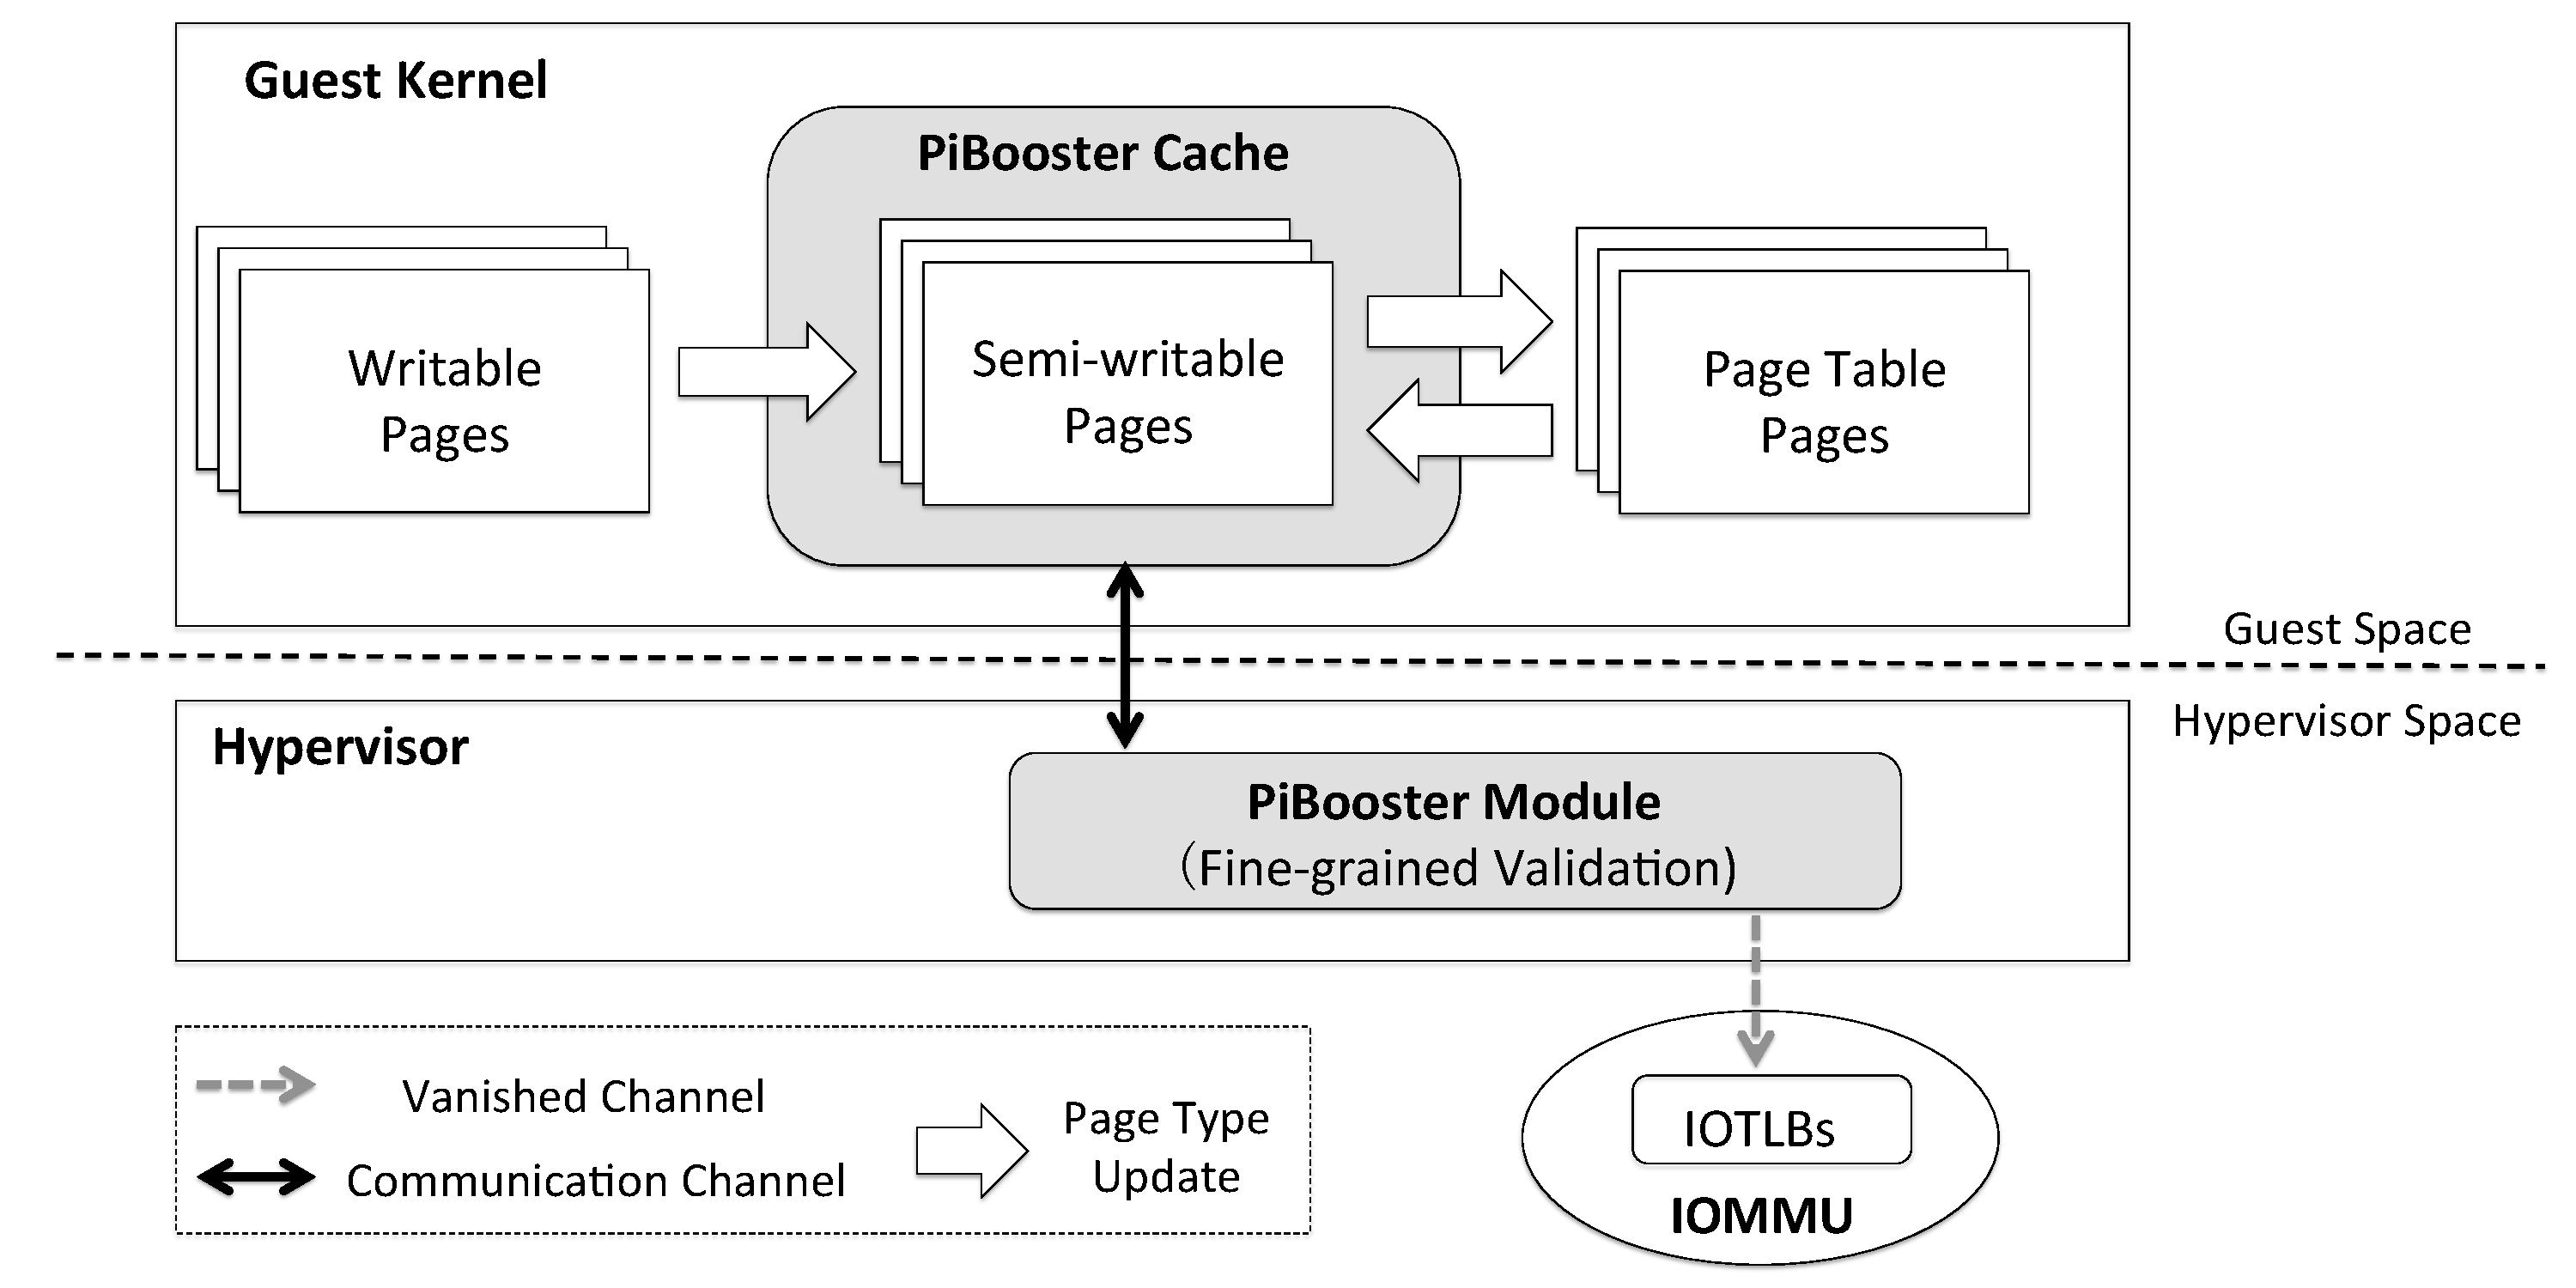
\includegraphics[width=0.8\textwidth]{image/overview/arch.pdf} \\
\caption{\name Architecture. The semi-writable pages are managed by the \name cache, and all page type updates are validated by the \name module.
Through the cooperation of \name cache and \name module, \name successfully shortens the execution path of the guest page table (de)allocation and eliminates additional IOTLB flushes.}
\label{fig:arch}
\end{figure*}

\subsection{Design Requirements}\label{sec:req}
In the design of \name, we consider several requirements, which are summarized and listed as follows.
\begin{enumerate}
\item Unaltered system security. The new scheme should not sacrifice the system security to obtain benefits from I/O performance. No one likes to use a system with known design loopholes.
\item Compatible with legacy applications. The new scheme should limit the modifications on the guest kernel and the hypervisor, without any modifications on the existing applications.
\item Small modifications. The new scheme should minimize the development cost on the guest kernel and the hypervisor.
\item Minimizing additional IOTLB flushes. The new scheme should minimize the number of IOTLB flushes, such as reducing the number to zero.
\end{enumerate}

\subsection{\name Architecture}
Figure~\ref{fig:arch} depicts the architecture of \name. It consists of a \cache in the guest kernel and a \name module in the hypervisor space.
%the mechanism of the \cache
The \cache allocates a number of semi-writable pages at the initial stage,  which are newly introduced by the fine-grained validation scheme (Section~\ref{sec:fine-grained}).
These semi-writable pages are maintained in a dedicated cache.
At runtime, the \cache is able to satisfy all page table allocation and deallocation requests, shortening the execution path and saving the time.
During these periods, there are many page type updates from/to the semi-writable pages.
The \cache mediates these updates and issues hypercalls to the hypervisor, asking it to perform the fine-gained security validations on the update requests.
Once the verified pages pass the validations, their page types will be updated accordingly.
%The guest kernel cannot bypass the security validation process, as the hypervisor is the only one to determine/update the page type.

The \module enforces the fine-grained validation scheme on the page table updates.
It performs (1) the page table validations that validate the page table contents as well as the type count, and (2) the DMA validations that ensure that the DMA requests cannot write the page-table pages and the semi-writable pages.
In the original validation scheme, the DMA validations always triggers the additional IOTLB flushes due to the access permission updates between the writable pages and the page-table pages.
In the fine-grained validation scheme, both the semi-writable page and the page-table page are non-writable for DMA requests.
Thus, the hypervisor never needs to do the IOTLB flushes or IOMMU page table updates, which will save the time of the whole security validation.
Moreover, it also further reduces the execution time of the page table allocations and deallocations.

\subsection{Fine-Grained Validation}\label{sec:fine-grained}
%To reduce the number of the IOTLB flushes, a possible approach is to let the hypervisor to manage the page table in its own space.
%In this way, there is no need for flushing IOTLB, but it will dramatically increase the size of the hypervisor, and consequently reduce the system security level.
%Another possible approach is to do the IOTLB flushing in a batch, meaning flushing multiple IOTLB entries all in one, instead of flushing them one after another.
%This approach is able to retain the system security, but it could not eliminate the IOTLB flushes, only reducing the number of IOTLB flushes in a certain level.
%In addition, this approach may result in security loopholes as the IOTLB entries are not synchronized with the corresponding IOMMU page table slots.

We attempt to solve this problem in a smart way, which could reduce the number of IOTLB flush to zero with only small modifications of the guest kernel and the hypervisor,
as well as retaining the system security.
In general, our approach is proposing a fine-grained security validation to replace the old and coarse-grained one doing page-table and DMA validation together.
Specifically, we observe that the original coarse-grained access control is the all-or-nothing style. i.e., the writable page is simultaneously writable for both software and DMA (device) while all other page types are non-writable for both software and DMA.
%In short, there ere only two types of pages: 1) \emph{writable page} and 2) \emph{non-writable page} (including three page-table page types and two segment descriptor page types), and their access permissions are mutually exclusive from each other.
%Thus, the page-type changing between them inevitably triggers the additional IOTLB flushes, otherwise there will be a security loophole.
To address this conflict without sacrificing the system security, we propose to create a new page type: \emph{semi-writable page}, which is writable for software but non-writable for DMA,
and require that the page type updates between the writable page and the page-table page must go through the semi-writable page first.
%In practice,  we can further restrict that the system only updates the page-table pages to/from the semi-writable pages and holds the semi-writable pages to stop them converting back to the writable pages.
since the semi-writable page and page-table page are already inaccessible to DMA, there is no need to do IOTLB flushes, meaning the additional IOTLB flushes could be totally avoided.
In order to facilitate the management of the semi-writable pages, we propose a cache, called \cache, in the guest kernel, and extend the existing page management data structure in the hypervisor space.
Similar to the management of the page-table pages, the hypervisor is only responsible for the final validation of the semi-writable page, leaving all other management operations for the \cache.
By doing this, we can keep the modifications as small as possible by reusing existing validation process and page-table management subsystem, and also retain the system security.

1) bad impacts of original coarse-grained validation scheme 1) additional IOTLB flushes, and 2) long validation process

2) How to do the fine-grained validation 1) semi-writable page 2) new page type updates 3) why save time and eliminate IOTLB flushes
\subsection{\name Module}\label{sec:module}
1) mark semi-writable page using new bits/flag

2) keep the page-table validations, update the DMA update process

3) new hypercalls for \cache

\subsection{\name Cache}\label{sec:cache}
The basic idea behind the \cache is to have caches of semi-writable pages available for page table allocations and deallocations.
Without the page oriented \cache, the kernel will spend much of its time allocating, initializing and freeing page-table pages.
The slab allocator that is similar to the \cache is not used in our settings, due to the following reasons.
First, it violates one of security requirements of the page-table pages enforced by the hypervisor.
In particular, the type count should be zero when a page is updated among the writable page, the semi-writable page and the page-table page.
However, the pages in the slab allocator are not always satisfy this restriction, leading to the exceptional crashes.
Second, the existing size-oriented management does not distinguish the page-table page with other pages that have the same size, and we believe the customization of this management mechanism would need lots of development costs, such as interface updates, internal data structure updates.
In addition, the related components that rely on the slab allocators may also be affected.
At last, adding the fine-grained validation mechanism only for one object (i.e., page-table page) will subvert the generality of the slab allocator.
Considering the above three reasons, we give up reusing the existing slab allocator and aim to build a dedicated one, called \cache, for page table allocation and deallocation.

\subsubsection{\name Cache Initialization and Destruction}
The \cache is enabled in the system bootup phase by default.
By doing so, the page tables of all user processes are maintained by the \cache from the very beginning.
To increase the flexibility, it is also allowed to dynamically enable it at runtime through the prepared interface.

In the initialization phase, the \cache allocates several pages from writable pages using existing system allocators, converts them into semi-writable pages, and maintains them in a dedicated cache list.
At runtime, the page table deallocations are always successful by efficiently pushing deallocated pages into the \cache.
When the guest kernel needs page-table pages, the \cache  will pop out the cached pages to satisfy the requirements.
In certain extremely cases (e.g., many allocation requests with a few or none of deallocations), if the cached pages are not enough for the request of a page table allocation, the \cache has to re-invokes the system allocators to get new ones.
Fortunately, the re-invocations are rarely happened in a workflow-stable system.
In fact, there are almost always several semi-writable pages in the \cache that are ready for page-table allocations after the system is running a few minutes in our experiments.

The \cache works in the whole life cycle of the guest by default, but the end  user is able to explicitly disable it at any time through the exported interface.
Once the \cache received the disable command, it will release all resources, e.g., deallocating the cached pages through the existing system allocators and releasing the data structures that are used for managing the cached pages.
In addition, it will also issue a hypercall to inform the hypervisor, which will disable the fine-grained validation mechanism and switch back to the original coarse-grained validation scheme.
%As the disable costs are quite high, we recommend that always keeping the \name running once it starts to work.

\subsubsection{Cache Shrinking}
When the memory management daemon (e.g., \emph{kswapd}) notices that memory is tight, it will explicitly call the exported interface of the \cache to free some memory.
%talk about the interface
There are two interfaces to shrink the cache pages. One is based on the page number. The memory management daemon can specify a number to ask the \cache to release.
The other one is based on the percentage. For instance, the kernel could ask the \cache to release 50\% cached pages.
%the size of the cache.
In fact, the number of semi-writable pages maintained in the \cache is not too much. In our experiments, it is always less than $180$, meaning the size of the cache is less than $720KB$.

The \cache could also automatically shrink itself through the predefined threshold.
The threshold can be defined according to the page number or the proportion (i.e., the number of the cached semi-writable pages over the number of the page-table pages), or the combination of them.
%In the current prototype, the threshold is the combination of the page number and the percentage.






